\documentclass[pagenumbers=false, paragraphafter=none]{goose-article}

\title{Microscopic prediction of stick-slip friction}
\author{Tom de Geus}
\hypersetup{pdfauthor={T.W.J. de Geus}}

\begin{document}

\twocolumn[
    \begin{@twocolumnfalse}
        \maketitle
    \end{@twocolumnfalse}
]
\sloppy

\paragraph{Impact.}

Understanding how slip at a frictional interface initiates is important for e.g.~earthquake prediction and precision engineering.
The force needed to start sliding a solid object over a flat surface is classically described by a ``static friction coefficient'': a constant established by measurements.
It was recently questioned if such constant exists, as it was shown to be poorly reproducible.

\paragraph{Model.}

A common model divides the interface in elastically interacting `blocks' that are elastic up to a certain threshold.
These thresholds are distributed as all contacts are different.
Different than commonly assumed, I argue that contacts have a finite size and therefore inertia.

\paragraph{Depinning.}

Without inertia, such model predicts a depinning transition.
The model corresponds to a $d$ dimensional interface driven over a disordered pinning potential by a $d + 1$ dimensional solid.
Below a critical driving force, the interface is pinned by disorder.
Above it, the interface moves at a constant velocity.
At the critical force, the interface is marginally stable and avalanches appear whose size diverges as a powerlaw, successfully reproducing some features of earthquakes.
Problematically, since elastic interactions between blocks are strictly positive (a failing block destabilises all other blocks) it has been shown theoretically that stick-slip is impossible: the system cannot build up ``overstress''.

\paragraph{Fracture.}

It is a known experimental fact that the system can build up an overstress before it fails catastrophically.
At this point, slip starts by a fracture-like object that unzips the interface, whose front velocity and surrounding stress field are well described by fracture mechanics.

\paragraph{How is an overstress build up?}

I argue that these two facts are not contradictory.
The effect of inertia, ignored in depinning, is consequential.
Blocks that come close to failure at the very end of a slip event have a high probability to be failed by the mechanical noise.
This results in an `armoured' interface that can build up an overstress.
With $x$ the distance to yielding locally, this corresponds to $P(x) \sim x^\theta$ with $\theta > 0$, but whose value depends on the surface roughness in some way.

\paragraph{Rheology.}

The effect of inertia is consequential in two more ways.
First, the failure of a block redistributes stress among neighbouring blocks by elastic waves.
Blocks thus receive transient stress overshoots causing them to fail prematurely such that they too emit waves.
This constitutes to a dynamic weakening such that the interface is \emph{velocity weakening}, well described by rate-and-state friction laws (blue curve).
Second, during the start of a slip event, the inertia of the surrounding elastic bulk provides a stabilising effect (quantified in the literature), such that the effective rheology is non-monotonic (red curve), with the minimum the ``dynamic friction coefficient'' denoted $f_c$.

\begin{figure}[htp]
    \centering
    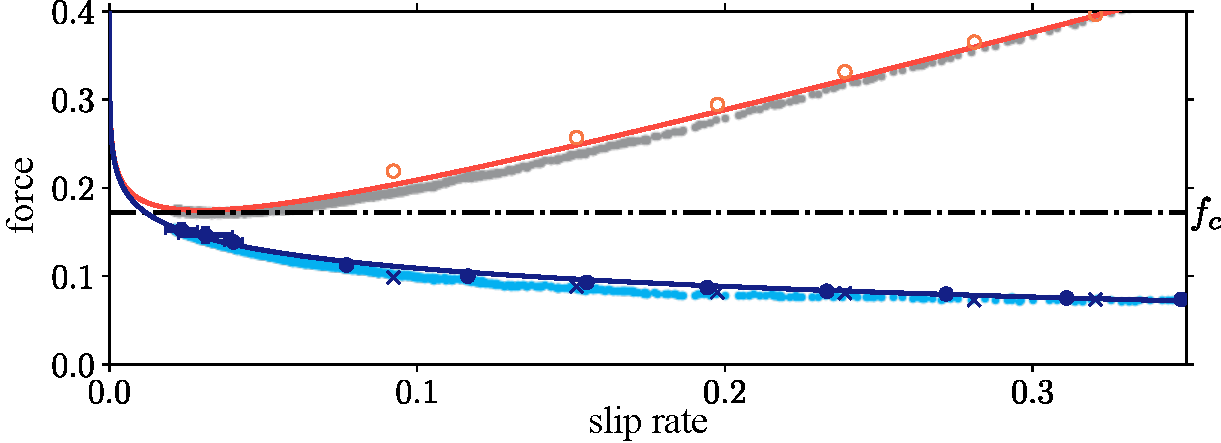
\includegraphics[width=\linewidth]{scenario.pdf}
\end{figure}

\paragraph{When does slip start?}

Due to the disorder $f_c$ varies in space.
Consequently, a microscopic event nucleated at $f_c$ can grow to a size $\ell$ with a finite probability, implying $P(\ell) \sim \ell^{-\tau}$ with $\tau > 0$.
At a load $f > f_c$ disorder can only stop a propagating avalanche if $l < l_c \sim | f - f_c |^{-\nu}$ (with $\nu$ related to the fluctuations of stress after slip).
However, due to the armouring, events are not numerous upon increasing the load ($\sim (f - f_c)^{\theta + 1}$) such that practically one observes a diverging avalanche scale $l_{\max} \sim (f - f_c)^{(\theta + 1) / (\tau -1)}$.
Slip happens when $l_{\max} \sim \l_c$, setting the ``static friction coefficient''.

\nocite{deGeus2022,ElSergany2023,deGeus2019}
\bibliographystyle{unsrtnat}
\renewcommand{\refname}{Selection of publications}
\bibliography{library}

\end{document}
